% \part{Equipment Tour}

\chapter{Overview}
\label{sec:eq_intro}

\section{Introduction}
\label{sec:eq_intro:intro}

The University of Virginia is part of the CMS experiment at CERN.  The CMS detector (\href{http://cms.web.cern.ch/cms/Detector/FullDetector/index.html}{website}) is a multistage general purpose detector.  It has four layers to detect different kinds of particles: The silicon tracker tracks the path of charged particles, the electromagnetic calorimeter (Ecal) measures the energy of electrons and photons, the hadron calorimeter measures the energy of hadrons, and the muon chambers tracks the path of muons to determine their energy.  UVA's main experimental efforts involve the Ecal.

The central cavity of CMS is cylindrical, with the beam coming in along its axis.  The walls of the cylinder are formed by the Ecal detectors.  The rounded walls are the barrel, and at either end are the endcaps.  The detectors are made of two main components.  The masses that react with the beam products are dense inorganic PbWO$_4$ (\textit{``lead-tungstate''}) scintillator crystals.  Behind those scintillators are the scintillation detectors.  In the barrel, these detectors are avalanche photodiodes (APDs).  In the endcap, these detectors are Vacuum Photo-Triodes (VPTs.)

Some of the main objectives of the CMS detector, such as the discovery of the Higgs boson, will be seen primarily in the Ecal.  If a light ($<$140\,GeV) Higgs boson is discovered, it will be from a H$^0$~$\to$~$\gamma + \gamma$ decay.  Above 140\,GeV and through 600\,GeV the Higgs boson is predicted to decay into two Z bosons, which further decay into four leptops, such as electrons and muons.  Electrons and photons will be detected by the Ecal.

\begin{figure}[htbp]
  \centering
  \parbox{0.75\textwidth}{\tiny
    Taken from K.W. Bell et al., ``\href{papers/1344324}{Vacuum Phototriodes for the CMS Electromagnetic Calorimeter Endcap},'' IEEE Transactions on Nuclear Science, vol. 51, no. 5, pp. 2284-2287, 2004.}
  \pgfimage[interpolate=true]{figures/ecal_cutaway}
  \caption{Schematic View of CMS Electromagnetic Calorimeter}
  \label{fig:eq_intro:ecal}
\end{figure}

As the beam comes in on-axis, the majority of the beam products are produced just off-axis.  This means that the endcaps receive the highest radiation dosage, and the detectors need to be especially hardened against neutron radiation.  The PbWO$_4$ crystals scintillate in the visible spectrum, near 420\,nm.   The faceplates of the VPTs are made of a radiation-hard UV-transmitting borosilicate glass.  Glass tends to darken when exposed to neutron radiation.  The glass used for the VPT faceplates is manufactured in small batches and is proven to have less than 10\,\% transmission loss after a dose of 20\,kGy over a 48\,hour period using a $^{60}$Co source, prior to being accepted for use in VPT production.

The exact performance characteristics of VPTs aren't yet fully understood, and the University of Virginia is performing exhaustive tests on their performance under the unique conditions at CMS.  UVA has previously studied their performance under temperature variation and their performance under non-axial magnetic fields (\secnameref{sec:eq_vpt:reading}.)

\section{Current Research}
UVA is currently (2010) studying the long term response behavior of VPTs in an axial magnetic field.  Previously, we've seen that the VPT's photocathode current decays over time in an exponential-like way.  This long-term decay behavior is being tested to determine if it follows an exponential decay, approaches one, or if some other function is needed to describe this behavior.  If the decline in photocathode current does approach an exponential decay, then VPT gain will approach zero over time.  If that happens, the decay needs to be determined, and a gain restoration technique must be implemented.

We've seen that VPTs return to their origianal gain once removed from the experimental setup and replaced some time later.  It remains to be seen if VPT gain can be restored electronically\dashem{}without removing them from the magnetic field, which cannot be done at CMS.

\section{Experimental Setup}
\label{sec:eq_intro:setup}

The experimental setup at UVa has two main sections: The \Gls{PXI Crate} and the \Gls{rig}.  The \gls{PXI Crate} sends signals from its \pxislottwo{}~\gls{FPGA} module to the rig's \glspl{LED board}.  The boards send a photon pulse to VPTs housed inside a 3.8\,T magnetic field, and the VPT translates those photons into a charge on its anode.  The anode signal is amplified by a Stephenson amplifier, and that amplified signal is sent back to the PXI Crate's \pxislotn{3}~Switch.  The PXI Crate then processes and records the signals.

Conceptually part of the rig, a high voltage supply provides a +800\,V and +600\,V potential difference to the VPT's anode and dynode, respectively.  A low voltage supply provides power to the LED pulser boards and the Stephenson amplifier.

Figure \ref{fig:eq_intro:rig_connections} is a conceptual view of the conduits between the components of the rig.  The ``Amp'' branch is a simplification.  Only the VPT anode connects to the amp, which then connects to the \pxislotn{7} Switch.  The VPT cathode bypasses the amp and connects to the \pxislotn{3} Switch.  The PIN diode (\secnameref{sec:eq_intro:vpt_branch}), part of the VPT node here, also bypasses the Amp to connect to the \pxislotn{7} Switch.

\begin{figure}[htbp]
  \centering
  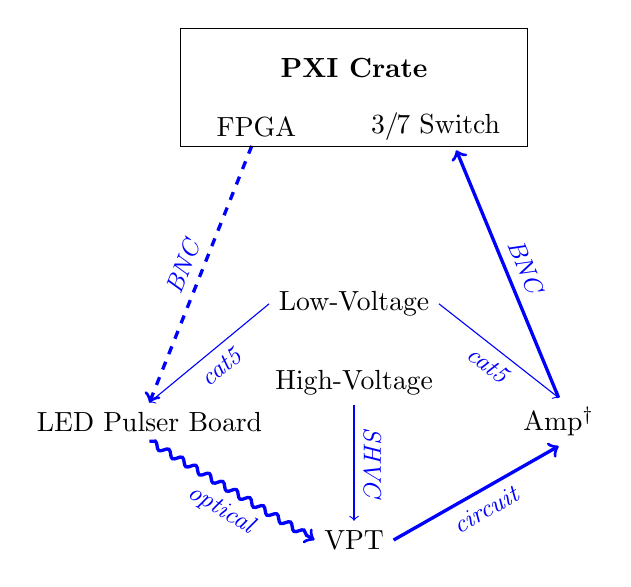
\begin{tikzpicture}
    
    \node (vpt) at (0,0) {VPT};
    \node (led) at (150:3) {LED Pulser Board};
    \node (amp) at (30:3) {Amp$^\dagger$};
    \node (hv)  at (90:2) {High-Voltage};
    \node (lv)  at (90:3) {Low-Voltage};
    \node (pxi) at (90:6) {\bfseries PXI Crate};
    \path (pxi) node (switch) at +(-30:1.5) {\hspace{-1.5em}\pxislotn{3}/\hspace{-.2ex}\pxislotn{7}\ Switch};
    \path (pxi) node (fpga)   at +(210:1.5) {\pxislottwo\ FPGA};

    \begin{scope}[blue]
    \path[->] (fpga.south) edge[dashed,very thick]
                                        node[above,sloped] {\itshape\small BNC}      (led.north);
    \path[->] (led.south)  edge[very thick,decorate,decoration={snake,amplitude=.4mm,segment length=2mm,post length=1mm}]
                                        node[below,sloped] {\itshape\small  optical} (vpt.west);
    \path[->] (vpt.east)   edge[solid,very thick]
                                       node[below,sloped] {\itshape\small  circuit} (amp.south);
    \path[->] (amp.north)  edge[solid,very thick]
                                        node[above,sloped] {\itshape\small  BNC}     (switch.south);
    \path[->] (lv.west)    edge[thin]   node[below,sloped] {\itshape\small  cat5}    (led.north);
    \path[->] (lv.east)    edge[thin]   node[below,sloped] {\itshape\small  cat5}    (amp.north);
    \path[->] (hv.south)   edge[thin]   node[above,sloped] {\itshape\small  SHVC}    (vpt.north);
    \end{scope}

    \draw (pxi) ++(-90:1) ++(left:2.2) rectangle ++(4.4,1.5);
    
  \end{tikzpicture}
\\\footnotesize $\dagger$\quad Conceptual node; anode only
  \caption{Rig Connections}
  \label{fig:eq_intro:rig_connections}
\end{figure}

\subsection{LED Branch}
\label{sec:eq_intro:led_branch}

The FPGA sends three TTL signals to a set of powered line driver chips (\model{74LS241N} and \model{74LS241PC}), which then drives the TTL signals over BNC cables to the powered LED board.  Each TTL signal corresponds to a single LED. (\secnameref{sec:eq_led})

\begin{labelled}{pxilabelled}
\item [Load Signal] is a simple simulated collider beam signal, intended to represent photon activity during beam events.
\item [Soak Signal] is a faux load between beam events to maintain the VPT's response curve.
\item [Reference Signal] is a measurement pulse inserted between the load and soak pulses to measure the VPT's response characteristics.
\end{labelled}

Each of the three optical signals that the LED board emits are multiplexed (muxed) into five different optical fibers, and terminate in light-sealed boxes containing a VPT and a PIN diode.  The PIN diode's signal can be used to make adjustments do to variations in LED light output on a pulse-by-pulse basis.  The light from each fiber is projected onto the entirety of the VPT's photocathode.  So, in total, each VPT receives three fibers (one from each LED), and there are five PIN diodes (one for each VPT) acting as references for LED light output.  


\begin{figure}[htbp]
  \centering
  \begin{tikzpicture}
  [  node distance=15mm,
     text height=1.2ex,
     text depth=.25ex,
  nonterminal/.style={
    rectangle, minimum size=6mm,
    very thick, draw=red!50!black!50,
    top color=white,
    bottom color=red!50!black!20,
    font=\itshape
  }, terminal/.style={
    rectangle, minimum size=6mm, rounded corners=3mm,
    very thick, draw=black!50,
    top color=white, bottom color=black!10,
    font=\ttfamily
  }, skip loop/.style={to path={-- ++(0,#1) -| (\tikztotarget)}}
  ]

  \node (fpga) [nonterminal] {{\normalfont\pxislottwo}\ FPGA};
  \node (led)  [terminal,right=of fpga] {LED Board};
  \node (vpt)  [terminal,right=of led,
                rectangle split, rectangle split parts=2, draw] {
                  VPT
                  \nodepart{second}
                  PIN
                };
  \node (amp)  [terminal,right=of vpt] {Amp};
  \node (hs)   [nonterminal,above=of amp] {{\normalfont\pxislotn{7}} Switch\ };
  \node (ls)   [nonterminal,below=of amp] {{\normalfont\pxislotn{3}} Switch\ };
  \node (sys)  [nonterminal,right=of amp] {{\normalfont\pxislotone} System Controller\ };
  \node (osc)  [nonterminal,above=of sys] {{\normalfont\pxislotn{6}} Oscilloscope\ };
  \node (dmm)  [nonterminal,below=of sys]  {{\normalfont\pxislotn{5}} DMM\ };

  \node (humiter) [terminal,left=of ls] {Humiter};

  \path[font=\small]

        (fpga.east)        edge[->]                node [above] {\itshape load} (led.west)
        ($(fpga.north east)!.25!(fpga.south east)$)
                          edge[->,out=60,in=120]   node[sloped,above]{\itshape reference}
                                                   ($(led.south west)!.75!(led.north west)$)
        ($(fpga.north east)!.75!(fpga.south east)$)
                          edge[->,out=-60,in=240]  node[sloped,above]{\itshape soak}
                                                   ($(led.south west)!.25!(led.north west)$)

        (led.east)        edge[->,very thick]      node [above] {\itshape load} (vpt.west)
        ($(led.north east)!.25!(led.south east)$)
                          edge[->,very thick,out=60,in=120]
                                                   node[sloped,above]{\itshape reference}
                                                   ($(vpt.south west)!.66!(vpt.north west)$)
        ($(led.north east)!.75!(led.south east)$)
                          edge[->,very thick,out=-60,in=240]  
                                                   node[sloped,above]{\itshape soak}
                                                   ($(vpt.south west)!.33!(vpt.north west)$)

        % (led.north)       edge[->,skip loop=5mm]   node [below] {\itshape soak}
        %                                            ($(vpt.north west)!.25!(vpt.north east)$)
        % (led.south)       edge[->,skip loop=-5mm]  node [below] {\itshape reference}
        %                                            ($(vpt.south west)!.25!(vpt.south east)$)
        ($(vpt.north west)!.75!(vpt.north east)$)
                          edge[->,skip loop=15mm,out=90,in=180,very thick]
                                                   node[sloped,above]{\itshape{}PIN}
                                                   (hs.west)
        (vpt.east)        edge[->,very thick]      node[sloped,above]{\itshape{}anode} (amp.west)
        (amp.north)       edge[->,very thick]      node[sloped,above]{\itshape{}anode} (hs.south)
        ($(vpt.south west)!.75!(vpt.south east)$)
                          edge[->,skip loop=15mm,out=-90,in=180,very thick]
                                                   node[sloped,below,pos=.35]{\itshape{}cathode}
                                                   ($(ls.north west)!.33!(ls.south west)$)
        ($(humiter.north east)!.66!(humiter.south east)$)
                         edge[->]
                                                   ($(ls.north west)!.66!(ls.south west)$)
        (ls.east)        edge[->]                  (dmm.west)
        (hs.east)        edge[->]                  (osc.west)
        (dmm.north)      edge[->]                  (sys.south)
        (osc.south)      edge[->]                  (sys.north);

  % LEGEND
  % \draw[help lines] (current bounding box.north west) rectangle (2em, 10em);
  \begin{scope}[node distance=3mm,font=\small]
    \node (space) [above=of fpga] {};
    \node (legend single)   [above=of space] {};
    \node (legend single 2) [right=of legend single,anchor=west] {\tiny Single Cable};
    \node (legend double)   [above=of legend single] {};
    \node (legend double 2) [right=of legend double,anchor=west] {\tiny Multiple Cables};
    \path
      (legend single)    edge[->]            (legend single 2)
      (legend double)    edge[->,very thick] (legend double 2);
  \end{scope}
\end{tikzpicture}

%%% Local Variables: 
%%% mode: latex
%%% TeX-master: "../Manual"
%%% End: 

  \caption{Signal Path in Teststand}
  \label{fig:eq_intro:signal}
\end{figure}

\subsection{VPT Branch}
\label{sec:eq_intro:vpt_branch}
A VPT (\secnameref{sec:eq_vpt}) is a single stage photomultiplier.  The VPT's photocathode, dynode, and anode accumulate charge as light impacts the photocathode, with the most charge accumulating on the anode.  As photons  strike the photocathode, electrons are liberated.  A large potential of $+600$\,V is driven from the photocathode to the dynode.  The current from the VPT's anode goes through an amplification stage, then both the anode and cathode are ultimate routed to the crates DMM or oscilloscope.

%  The current from the VPT's anode goes through an amplifier (\secnameref{sec:eq_preamp}) before being routed to the crate's \pxislotn{7} high-frequency switch, then to the \pxislotn{6} oscilloscope.  The PIN diode connects the same way, but unamplified.  The VPT's cathode is instead connected to a distribution box near the crate, which connects a terminal block on the crate's \pxislotn{3} low-frequency switch, then to the \pxislotn{5} DMM.

The VPT's anode is connected directly to an amplifier circuit (\secnameref{sec:eq_preamp}), which connects to the \pxislotn{7} high-frequency switch.  The PIN diode signal passes unmodified to that same \pxislotn{7} high-frequency switch.  The cathode signal cables connect to a distribution box near the PXI Crate.  The distribution box then routes their signals to the terminal block on the \pxislotn{3} low-frequency switch.  All of these signals leave the rig over \gls{BNC} cables before terminating at or adjacent to the PXI Crate.

\begin{figure}[htbp]
  \centering
  \pgfimage[interpolate=true,height=3in]{figures/IMG_0093}
  \caption{Distribution Box for Cathode Signal to Terminal Block}
  \label{fig:eq_intro:distribution_box}
\end{figure}

A temperature and humidity monitor (\gls{humiditer}) is mounted next to the rig, and a single cat5 cable carries power to it and returns its readings to the \pxislotn{3} low-frequency switch via the distribution box. It connects via \Gls{Molex} connector next to the cathode signal \gls{BNC} connectors.

\section{Triggering}

Trigger logic is contained in the FPGA VI and in \path{Main.vi}.  The FPGA VI contains a loop for each LED which waits for input from the \path{Main.vi}.  Once it receives input it sets the LED line high and goes into a 25\,ns subloop and checks the time until the period of the frequency set by \path{Main.vi} has elapsed, then sets the LED line low.  The real frequency is then calculated and returned to \path{Main.vi}.

\section{Analysis}

The data needs to be cleaned up before processing.  This includes excluding statistical outliers.  Anode and cathode measurements need to be corrected for experimental variations.  Variations in light are represented by variations in PIN diode measurements.  Amplifier variablity can be measured with a test signal, but this is offline for the current measurements, because the cables used for this measurement were picking up radio interference.  The anode data points then need to be corrected for amplifier variability.  A large amount of data is collected, and it is currently averaged to 15 data points every 45 minutes.  The cleaned data is then ready for visualization and statistical analysis.


%%% Local Variables: 
%%% mode: latex
%%% TeX-master: "Manual"
%%% End: 
